\section{Time box 3}
\subsection{Time box planning}
Overview of the what work is put into which time boxes.
\begin{figure}[H]
	\begin{centering}
		 %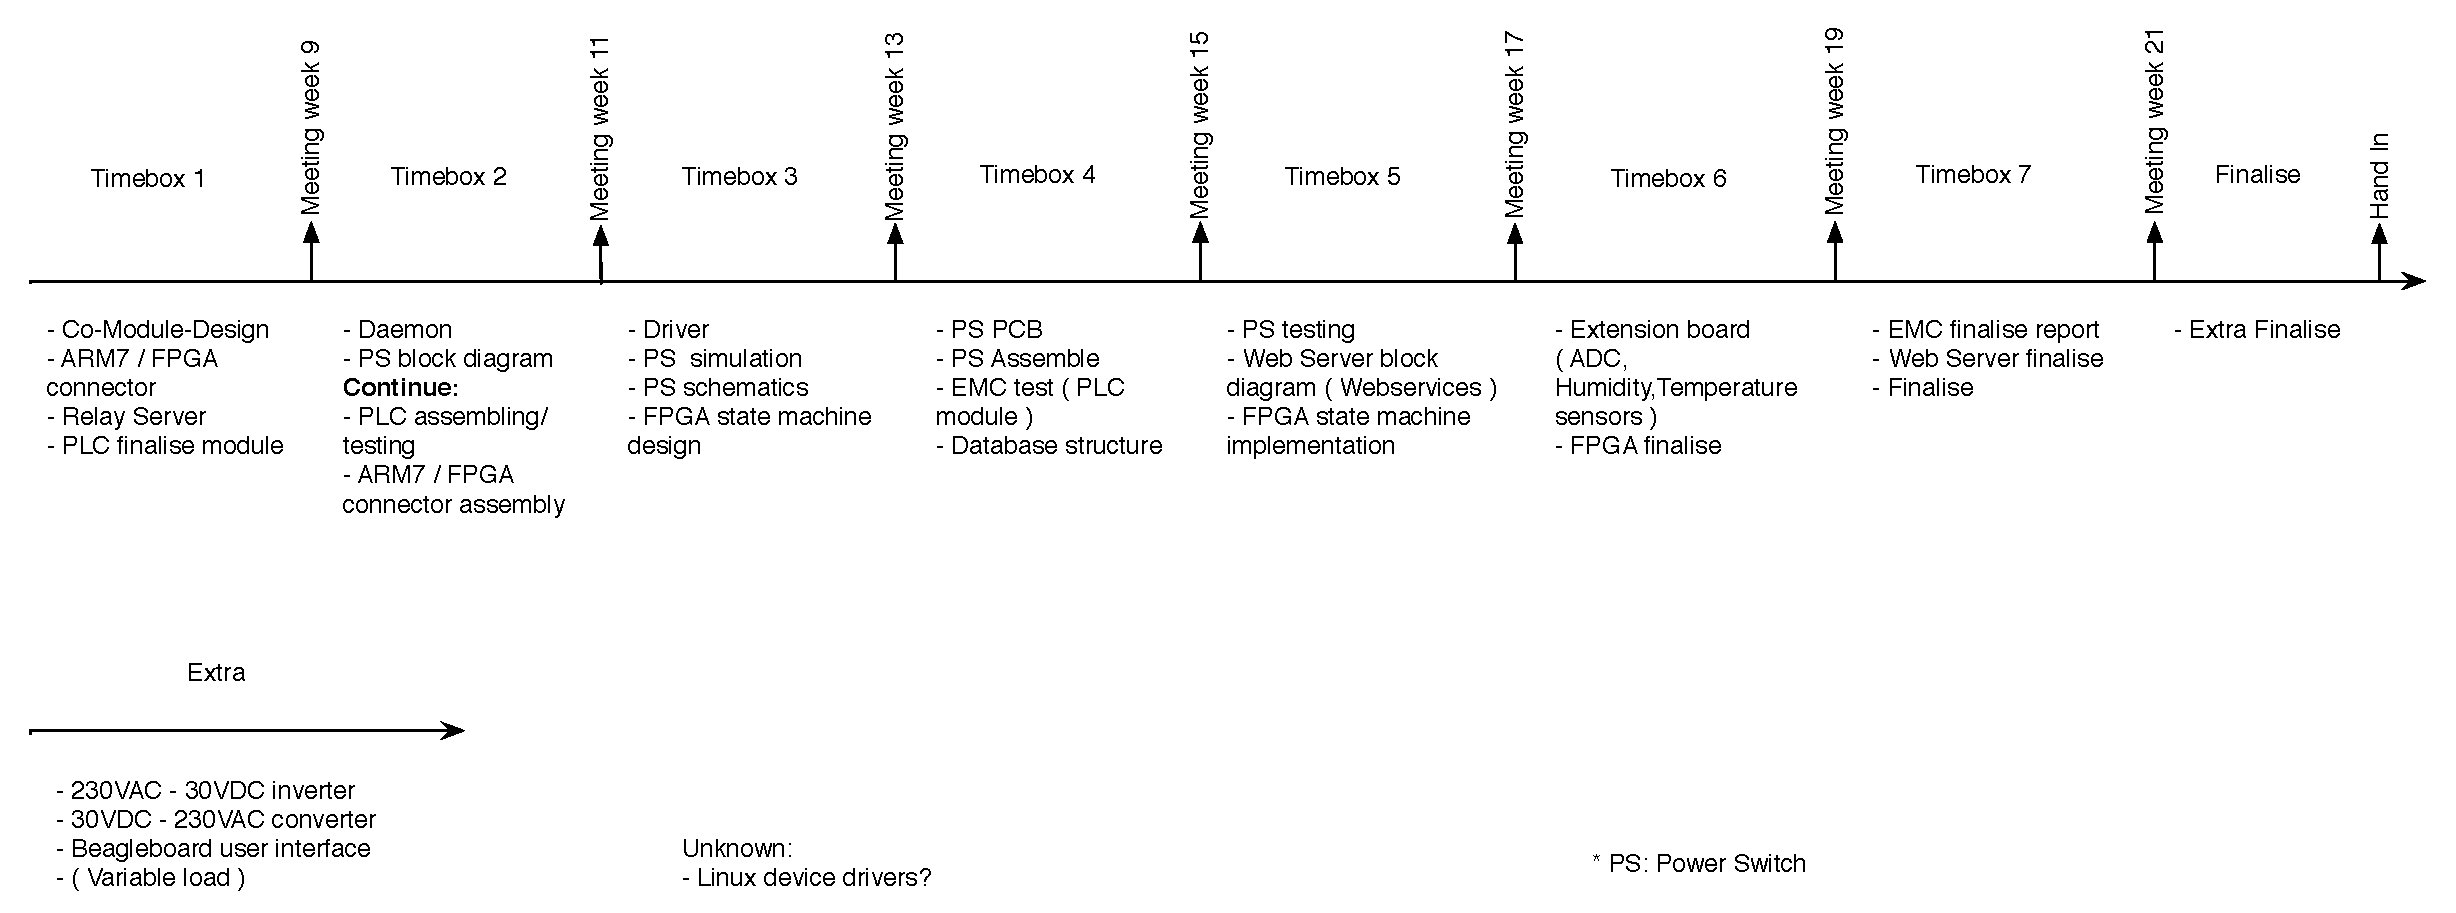
\includegraphics[width=1.0\textwidth]{images/tb_r2.pdf}
		%\caption{Updated time-box}
		\missingfigure{Updated timeline}
	\end{centering}
\end{figure}

\subsubsection{Work to be done in this time box}
\begin{itemize}
	\item Power switch
	\begin{itemize}
		\item Schematic
		\item Printed circuit board
		\item Mount component
		\item Test board
	\end{itemize}
	\item Host controller
	\begin{itemize}
		\item Master wishbone
		\item CPU interface
	\end{itemize}
\end{itemize}
\paragraph{Description:}
\begin{description}
	\item[Power switch] A single switch port board for the power switch has to be made, as an essential part for the power switch
	\item[Host controller] is made in the FPGA, and is responsible for the communication between the Spartan6 and the ARM7, it shall be made with wishbone master interface 
\end{description}

\subsection{Power switch}

\subsection{Host controller}
The host controller takes commands from the ARM7, and controlling blocks in the Spartan6. This controller is made in hardware and implemented in the Spartan6.
\begin{figure}[H]
	\begin{centering}
		 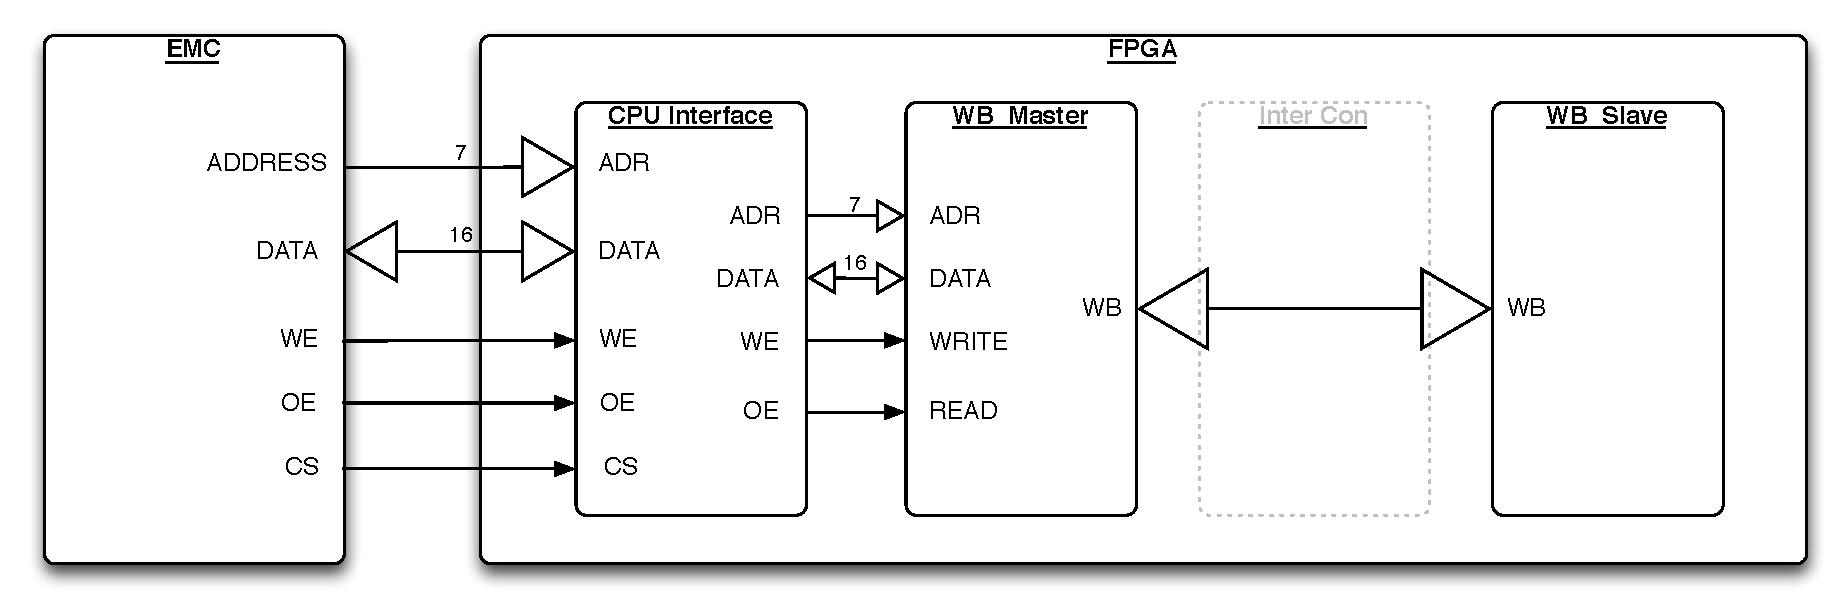
\includegraphics[width=1.0\textwidth]{images/host_controller.pdf}
		\caption{Host controller}
		%\missingfigure{host controller diagram}
	\end{centering}
\end{figure}
\subsubsection{External memory controller}
The EMC is a memory controller peripheral that support asynchronous static memory device such as RAM, ROM and flash. The chip select is used to select which memory device the AMR7 wants to communicate with. A block diagram of the EMC is shown below.
\begin{figure}[H]
	\begin{centering}
		 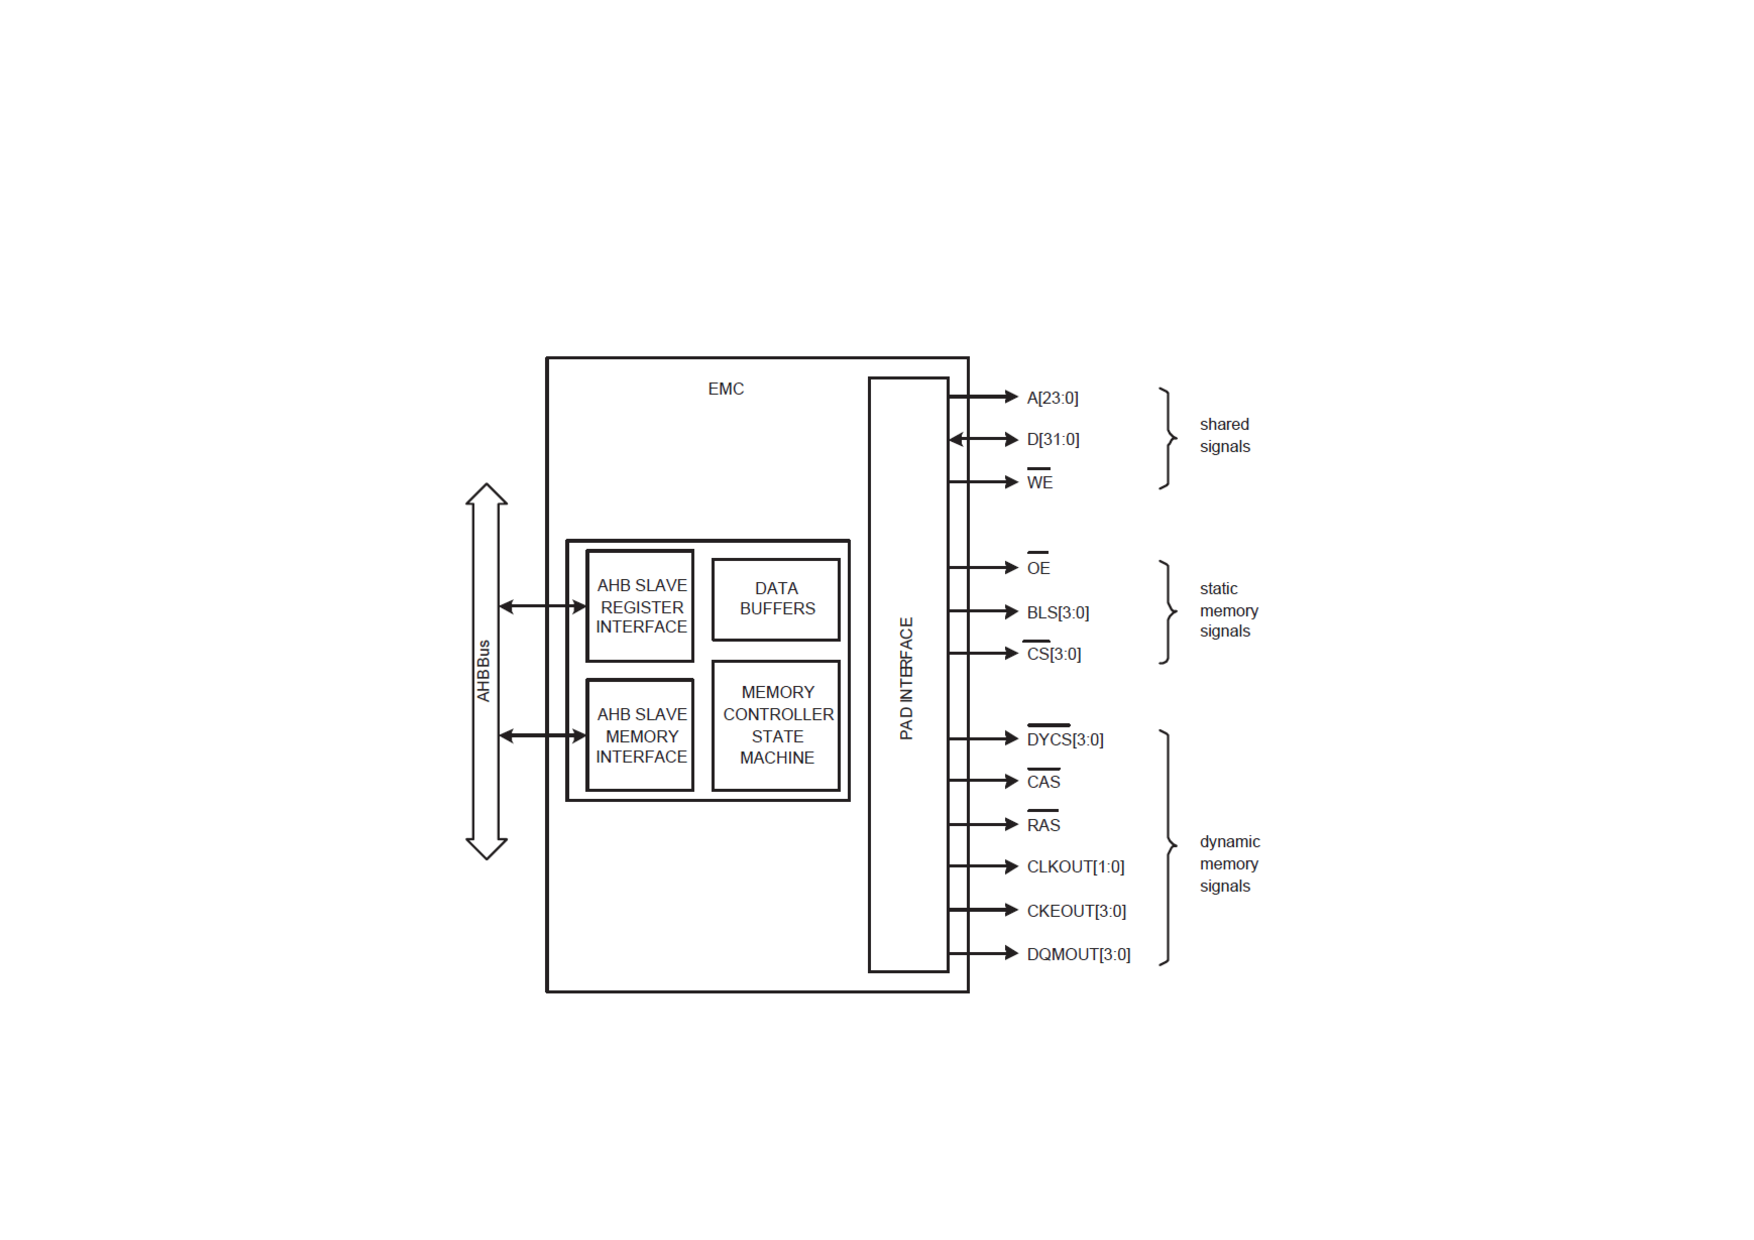
\includegraphics[width=0.7\textwidth]{images/emb_block_diagram.pdf}
		\caption{EMC block diagram}
		%\missingfigure{host controller diagram}
	\end{centering}
\end{figure}
The EMC is used to communicate with the Spartan6 board, with a 7 bit address and a 16 bit data bus, plus a read, write and chip select signal to indicate if it wants to read or write data, and select that it is the Spartan6 it would like data from. In this project the EMC is only used in static mode without the byte lane selects. A diagram of the EMC block is shown below.
\subsubsection{CPU interface}
The CPU interface communicate with the EMC on one site and with the master wishbone on the other site. The purpose of this interface is to determine if the EMC wants to communicate with the Spartan6, and if the ARM7 wants to read or write data.

\begin{lstlisting}[language=VHDL]
process (Clk,Rst)
	begin  
		if Rst = '1' then								--Reset set everything to 0
			Wr_o	<= '0';
			Rd_o	<= '0';
			A_o		<= (others => '0');
			D_o		<= (others => '0');
			CpuD_o	<= (others => '0');
		elsif (Clk'event and Clk = '1') then
			if CpuCs_i = '1' then					--Check chip select
				A_o	<= CpuA_i;							--Adress routing
					if CpuRd_i = '1' then			--Reading
						Rd_o	<= CpuRd_i;
						Wr_o	<= CpuWr_i;
						CpuD_o	<= D_i;					--Wishbone data out to Cpu data input
					elsif CpuWr_i = '1' then	--Writing
						Wr_o	<= CpuWr_i;					
						Rd_o	<= CpuRd_i;
						D_o		<= CpuD_i;				--Cpu data output to wishbone data input
					else
						Wr_o	<= CpuWr_i;		
						Rd_o	<= CpuRd_i;
						D_o		<= CpuD_i;
						CpuD_o	<= (others => '0');
					end if;
			else													--If chip select not high everything is set to 0
				Wr_o	<= '0';	
				Rd_o	<= '0';
				D_o		<= (others => '0');
				A_o		<= (others => '0');
				CpuD_o	<= (others => '0');
			end if;
		end if;
end process;
\end{lstlisting}
The block is synchronous with the clock and have an asynchronous reset. If the reset is pressed everything is set to zero to tell the master wishbone to not do anything. When the chip select is high, it tells the block that the ARM7 want to communicate with the Spartan6. After chip select is activated, the block check if the ARM7 want to read or write data from or to the Spartan6. If the ARM7 wants to read data, the interface block route the data from master wishbone to the data vector on the EMC. Else if the ARM7 wants to write data, the data vector on the EMC is routed to the data input for the master wishbone. In any case of read or write the read and write output from the EMC is routed to the master wishbone. The address input from the EMC is routed as soon as the chip select is activated. If the chip select is not active everything is routed to zero, to secure that the master wishbone do not write any data. The data output to the EMC is tri-stated in the wrapper code if the chip select is not active, to not disturb other communication on the EMC bus.
\paragraph{Test bench}
The test bench is made to test if the host controller is responding correct to different signals, image of the test bench signals is shown below.
\begin{figure}[H]
	\begin{centering}
		 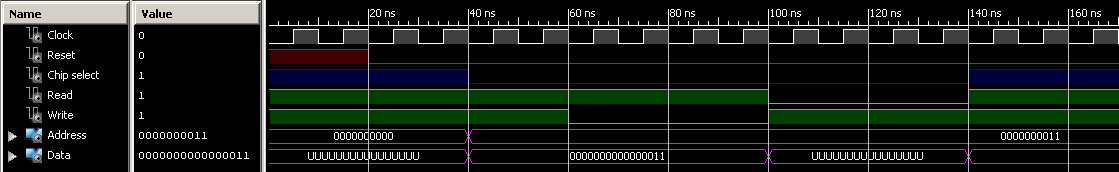
\includegraphics[width=1.0\textwidth]{images/host_controller_tb.png}
		\caption{Host controller test bench}
		%\missingfigure{host controller diagram}
	\end{centering}
\end{figure}
The test bench shows that after the reset state and when the chip select is active, a write cycle is made,to address "0x03" and the data that is written is "0x03". After the write there is made a read cycle on address "0x03" and the data read is uninitialized, this is because the master wishbone do not get any data from slave, so it is not possible to send any valid data to the ARM7, so the uninitialized indicate so far that the read cycle works. And after the chip select deactivate the data is equal to the data from the AMR7.
\subsubsection{Wishbone}

Wishbone is a computer bus for integrated circuit communication. It sets up some standard communication rules to use when designing IP cores. This make it easy to reuse code on different hardware and in different systems. The wishbone bus is a logic bus, this means that there is no rules for voltage levels, it only works with ones and zeros. In this project the wishbone is used as illustrated on the picture below.
\begin{figure}[H]
	\begin{centering}
		 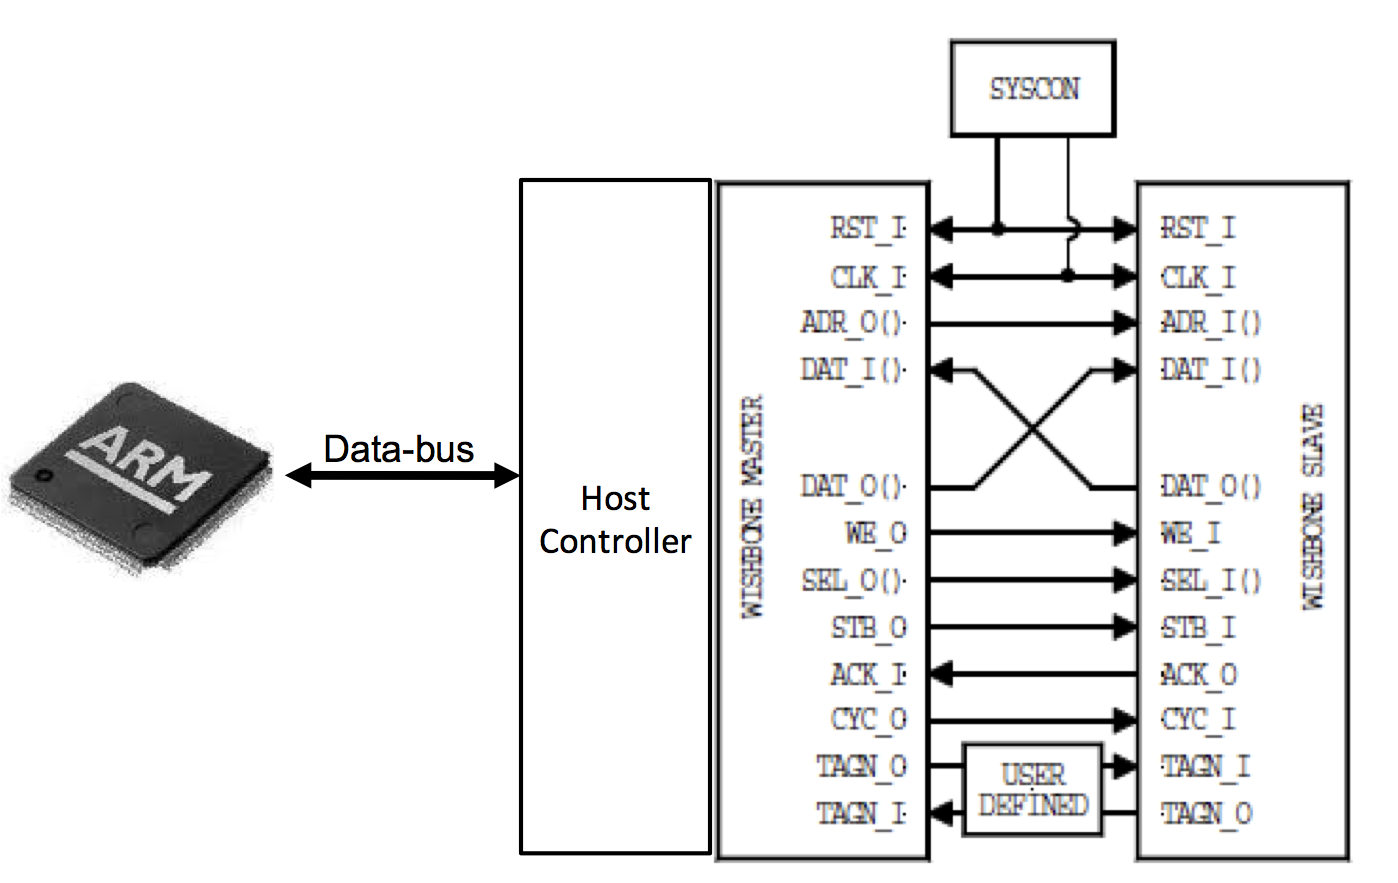
\includegraphics[width=0.8\textwidth]{images/typical_usage.png}
		\caption{Wishbone connection for the host controller}
		%\missingfigure{host controller diagram}
	\end{centering}
\end{figure}
The EMC on the ARM7 is controlling the wishbone master, which is controlling all the wishbone slaves that is in the system. This make it easier to write a driver for the ARM7 that controls the master wishbone through the EMC. Then the master wishbone control every IP core with at wishbone slave interface connected. In this project the wishbone is going to use single read and write cycles, the single read cycle timing diagram is shown below.
\begin{figure}[H]
	\begin{centering}
		 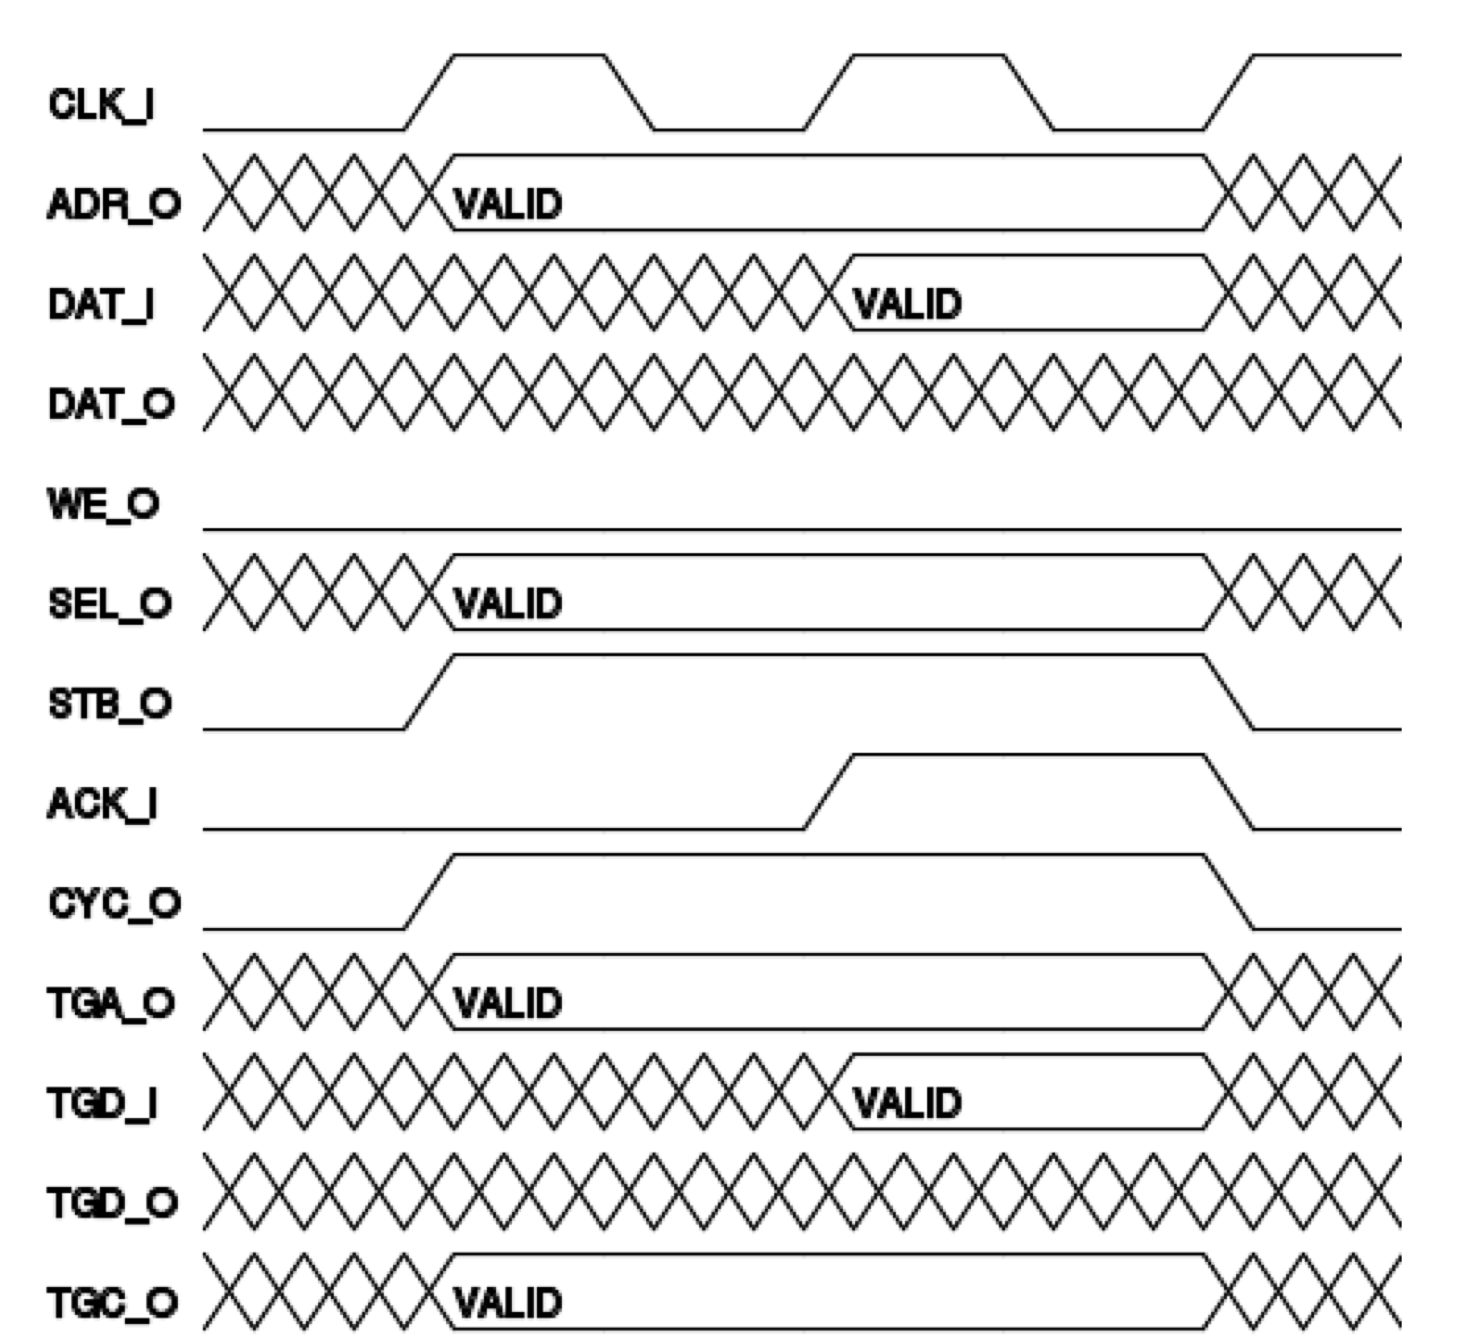
\includegraphics[width=0.65\textwidth]{images/wb_single_read.png}
		\caption{Single read cycle}
		%\missingfigure{host controller diagram}
	\end{centering}
\end{figure}
When a single read cycle is started, the master wishbone presents a valid address, on the address register, it set the write enable to zero to show that this is a read cycle, the SEL\_O is set, to show where on the data input it expect the data to be read, it also sets the CYC\_O and STB\_O high to indicate the start of a cycle and a phase.


On the next raising clock edge, the slave decode the input and set the acknowledge bit high in response to the SEL\_O. It also presents valid data on the slave data output. The master monitors the acknowledge and prepares to latch data.


On the third raising clock edge the master wishbone latches the data, and set the STB\_O and CYC\_O to zero to end the cycle and the phase, the slave set the acknowledge bit low again as response to STB\_O.\\
The timing diagram for the single write cycle is shown below.
\begin{figure}[H]
	\begin{centering}
		 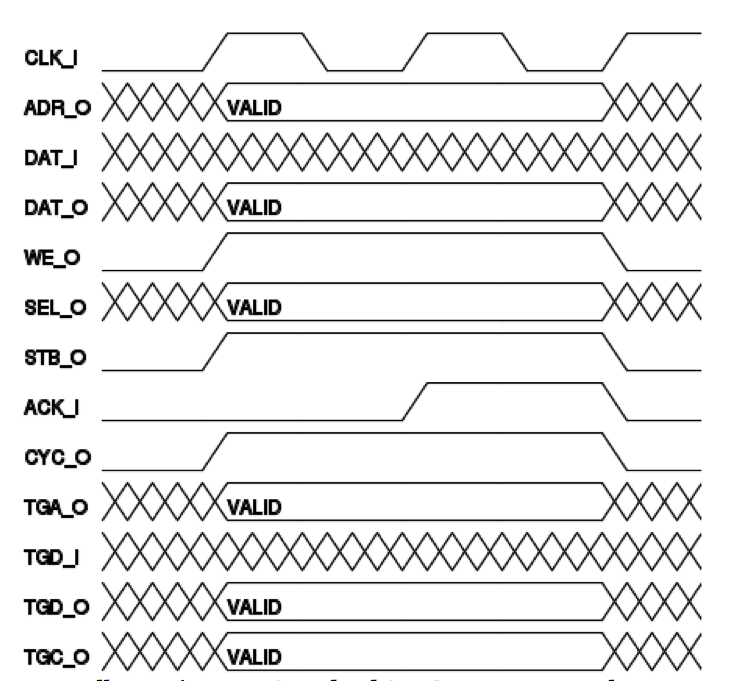
\includegraphics[width=0.65\textwidth]{images/wb_single_write.png}
		\caption{Single write cycle}
		%\missingfigure{host controller diagram}
	\end{centering}
\end{figure}
When the master wishbone wants to write to the slave, it present valid address and data on the address register and data output, it also sets the write enable high to indicate the cycle is write. As with the read the STB\_O and CYC\_O is set high to indicate cycle and phase start, all this is done on the first raising clock edge.

On the second raising clock edge the slave decode the input and set the acknowledge bit high in response to the SEL\_O. It also prepares to latch data from the master. The master monitors the acknowledge bit and prepare to terminate the cycle.

On the last raising clock edge the slave latches the data, the master set the STB\_O and CYC\_O to zero to end the cycle and the phase, the slave set the acknowledge bit low again as response to STB\_O.
\subsection{Post deployment}
Spend a short time evaluating the just-closed timebox. What went well? Why did it go well? What caused problems? Can they be prevented in the future? And how can they be prevented?
\subsubsection{Power switch}
\subsubsection{Host Controller}
The host controller work in theory but still needs to be tested in practice. The handed out code, was well commented to give a good overview. This made it easier to make the code for CPUinterface.